%========================================
% LESSON CONTENT: Ecuaciones Lineales en Dos Variables
%========================================

\lesson{Ecuaciones Lineales en Dos Variables}

%========================================
% SECTION 11.1: Introducción
%========================================
\subsectiontitle{Introducción a las Ecuaciones Lineales en Dos Variables}

\begin{definition}
\textbf{Ecuación Lineal en Dos Variables:}

Una ecuación lineal en dos variables es una ecuación que se puede escribir en la forma:

$$\boxed{Ax + By = C}$$

donde:
\begin{itemize}
    \item $A$, $B$ y $C$ son constantes (números reales)
    \item $A$ y $B$ no son ambos cero
    \item $x$ e $y$ son las variables
\end{itemize}

Esta forma se conoce como \textbf{forma estándar} de una ecuación lineal.
\end{definition}

\textbf{Ejemplos de ecuaciones lineales en dos variables:}
\begin{itemize}
    \item $2x + 3y = 6$ \quad (donde $A = 2$, $B = 3$, $C = 6$)
    \item $x - 4y = 8$ \quad (donde $A = 1$, $B = -4$, $C = 8$)
    \item $5x = 10$ \quad (donde $A = 5$, $B = 0$, $C = 10$)
    \item $-3y = 9$ \quad (donde $A = 0$, $B = -3$, $C = 9$)
\end{itemize}

\textbf{Observación importante:} A diferencia de las ecuaciones lineales con una variable (que tienen una solución), las ecuaciones lineales con dos variables tienen un \textbf{número infinito de soluciones}.

\newpage
%========================================
% SECTION 11.2: Soluciones y Gráficas
%========================================
\subsectiontitle{Soluciones y Gráficas de Ecuaciones Lineales}

\begin{definition}
\textbf{Solución de una Ecuación Lineal en Dos Variables:}

Una solución de una ecuación lineal en dos variables es un \textbf{par ordenado} $(x, y)$ que satisface la ecuación cuando los valores se sustituyen en ella.

Estas soluciones se pueden representar como \textbf{puntos} en el sistema de coordenadas rectangulares (visto en la Lección 10).
\end{definition}

\subsubsection*{Método de Tabulación}

Para encontrar soluciones de una ecuación lineal:
\begin{enumerate}
    \item Elija un valor para una de las variables (usualmente $x$)
    \item Sustituya ese valor en la ecuación
    \item Resuelva para la otra variable ($y$)
    \item El par ordenado $(x, y)$ es una solución
    \item Repita el proceso para obtener más soluciones
\end{enumerate}

\begin{example}
\textbf{Encontrar soluciones de una ecuación lineal}

Dada la ecuación $2x + 3y = 6$, encuentre al menos tres soluciones.

\textbf{Solución:}

\textbf{Para $x = 0$:}
\begin{align*}
2(0) + 3y &= 6 \\
3y &= 6 \\
y &= 2
\end{align*}
Solución: $(0, 2)$

\textbf{Para $x = 3$:}
\begin{align*}
2(3) + 3y &= 6 \\
6 + 3y &= 6 \\
3y &= 0 \\
y &= 0
\end{align*}
Solución: $(3, 0)$

\textbf{Para $x = -3$:}
\begin{align*}
2(-3) + 3y &= 6 \\
-6 + 3y &= 6 \\
3y &= 12 \\
y &= 4
\end{align*}
Solución: $(-3, 4)$

\textbf{Tabla de valores:}

\begin{center}
\begin{tabular}{|c|c|c|}
\hline
$x$ & $y$ & Punto $(x, y)$ \\
\hline
$-3$ & $4$ & $(-3, 4)$ \\
\hline
$0$ & $2$ & $(0, 2)$ \\
\hline
$3$ & $0$ & $(3, 0)$ \\
\hline
$6$ & $-2$ & $(6, -2)$ \\
\hline
$9$ & $-4$ & $(9, -4)$ \\
\hline
\end{tabular}
\end{center}
\end{example}

\newpage

\subsubsection*{Gráfica de una Ecuación Lineal}

\begin{theorem}
\textbf{Propiedad Fundamental:}

La gráfica de cualquier ecuación lineal en dos variables es una \textbf{línea recta}.

Para graficar una ecuación lineal:
\begin{enumerate}
    \item Encuentre al menos dos puntos (soluciones) de la ecuación
    \item Grafique estos puntos en el plano de coordenadas
    \item Trace una línea recta que pase por todos los puntos
\end{enumerate}

\textbf{Nota:} Aunque solo se necesitan dos puntos para definir una recta, es recomendable encontrar un tercer punto como verificación.
\end{theorem}

% Graphical representation of 2x + 3y = 6
\begin{center}
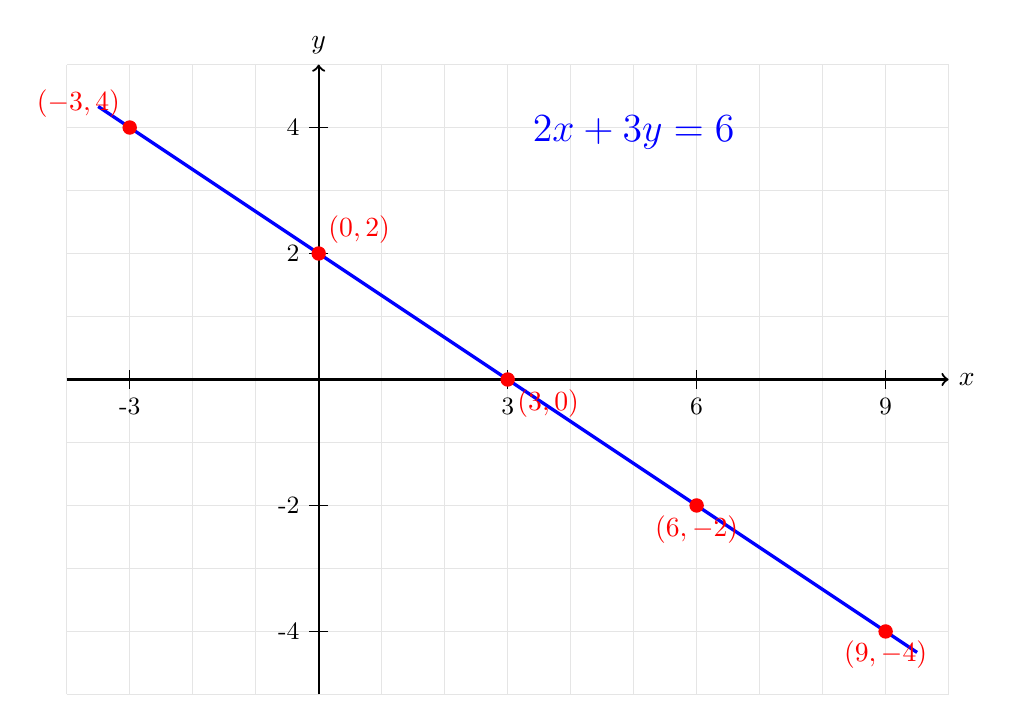
\begin{tikzpicture}[scale=0.8]
    % Grid
    \draw[gray!20, very thin] (-4,-5) grid (10,5);

    % Axes
    \draw[->, thick] (-4,0) -- (10,0) node[right] {$x$};
    \draw[->, thick] (0,-5) -- (0,5) node[above] {$y$};

    % Axis labels
    \foreach \x in {-3,3,6,9}
        \draw (\x,0.15) -- (\x,-0.15) node[below, font=\small] {\x};
    \foreach \y in {-4,-2,2,4}
        \draw (0.15,\y) -- (-0.15,\y) node[left, font=\small] {\y};

    % Plot the line 2x + 3y = 6
    \draw[blue, very thick, domain=-3.5:9.5] plot (\x, {(6-2*\x)/3});

    % Plot the points from table
    \filldraw[red] (-3,4) circle (3pt);
    \node[red, above left] at (-3,4) {$(-3,4)$};

    \filldraw[red] (0,2) circle (3pt);
    \node[red, above right] at (0,2) {$(0,2)$};

    \filldraw[red] (3,0) circle (3pt);
    \node[red, below right] at (3,0) {$(3,0)$};

    \filldraw[red] (6,-2) circle (3pt);
    \node[red, below] at (6,-2) {$(6,-2)$};

    \filldraw[red] (9,-4) circle (3pt);
    \node[red, below] at (9,-4) {$(9,-4)$};

    % Equation label
    \node[blue, above] at (5,3.5) {\Large $2x + 3y = 6$};
\end{tikzpicture}
\end{center}

\newpage
%========================================
% SECTION 11.3: Intersecciones con los Ejes
%========================================
\subsectiontitle{Intersecciones con los Ejes}

Las intersecciones con los ejes son puntos especiales que facilitan la gráfica de ecuaciones lineales.

\begin{definition}
\textbf{Intersecciones (Interceptos):}

\begin{itemize}
    \item \textbf{Intersección con el eje $x$ (x-intercept):} Las coordenadas $x$ de los puntos donde la gráfica interseca al eje $x$.
    \begin{itemize}
        \item Para encontrarla: Haga $y = 0$ y despeje $x$
        \item El punto tiene la forma $(a, 0)$
    \end{itemize}

    \item \textbf{Intersección con el eje $y$ (y-intercept):} Las coordenadas $y$ de los puntos donde la gráfica interseca al eje $y$.
    \begin{itemize}
        \item Para encontrarla: Haga $x = 0$ y despeje $y$
        \item El punto tiene la forma $(0, b)$
    \end{itemize}
\end{itemize}
\end{definition}

% Visual representation of intercepts
\begin{center}
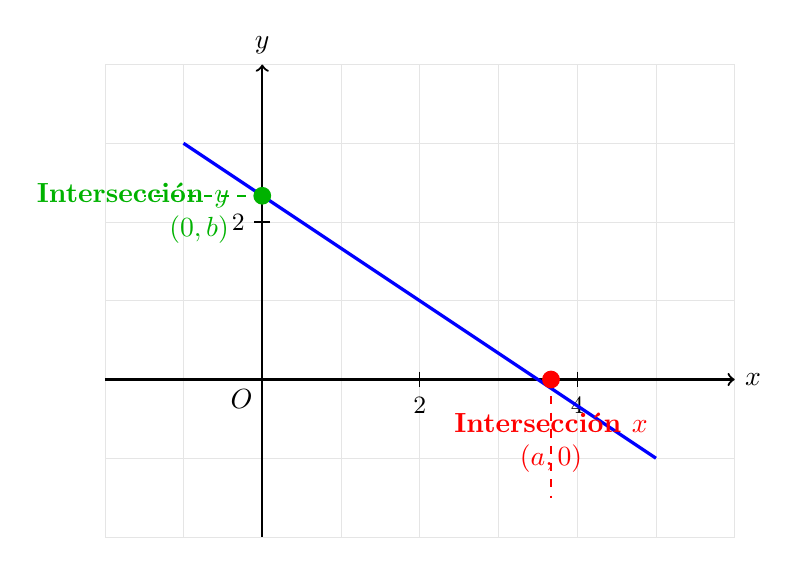
\begin{tikzpicture}[scale=1.0]
    % Grid
    \draw[gray!20, very thin] (-2,-2) grid (6,4);

    % Axes
    \draw[->, thick] (-2,0) -- (6,0) node[right] {$x$};
    \draw[->, thick] (0,-2) -- (0,4) node[above] {$y$};

    % Axis labels
    \foreach \x in {2,4}
        \draw (\x,0.1) -- (\x,-0.1) node[below, font=\small] {\x};
    \foreach \y in {2}
        \draw (0.1,\y) -- (-0.1,\y) node[left, font=\small] {\y};

    % Plot a line
    \draw[blue, very thick] (-1,3) -- (5,-1);

    % x-intercept
    \filldraw[red] (3.667,0) circle (3pt);
    \node[red, below] at (3.667,-0.3) {\textbf{Intersección $x$}};
    \node[red, below] at (3.667,-0.7) {$(a, 0)$};
    \draw[red, dashed, thick] (3.667,0) -- (3.667,-1.5);

    % y-intercept
    \filldraw[green!70!black] (0,2.333) circle (3pt);
    \node[green!70!black, left] at (-0.3,2.333) {\textbf{Intersección $y$}};
    \node[green!70!black, left] at (-0.3,1.9) {$(0, b)$};
    \draw[green!70!black, dashed, thick] (0,2.333) -- (-1.5,2.333);

    % Origin
    \node[below left] at (0,0) {$O$};
\end{tikzpicture}
\end{center}

\newpage
\begin{example}
\textbf{Encontrar las intersecciones con los ejes}

Para la ecuación $3x - 4y = 12$, encuentre las intersecciones con ambos ejes.

\textbf{Solución:}

\textbf{Intersección con el eje $x$ ($y = 0$):}
\begin{align*}
3x - 4(0) &= 12 \\
3x &= 12 \\
x &= 4
\end{align*}
Intersección con el eje $x$: $(4, 0)$

\textbf{Intersección con el eje $y$ ($x = 0$):}
\begin{align*}
3(0) - 4y &= 12 \\
-4y &= 12 \\
y &= -3
\end{align*}
Intersección con el eje $y$: $(0, -3)$

\textbf{Gráfica usando las intersecciones:}

\begin{center}
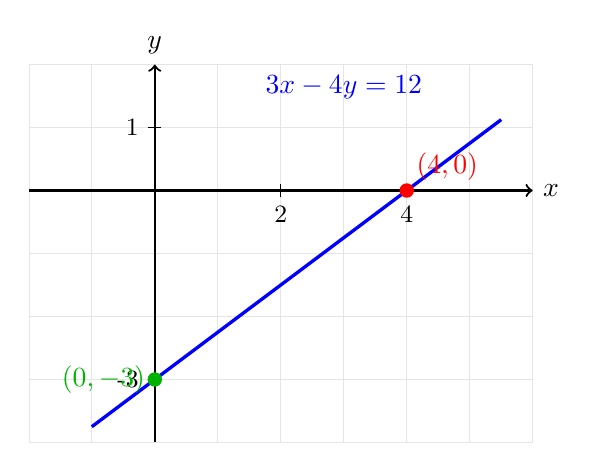
\begin{tikzpicture}[scale=0.8]
    % Grid
    \draw[gray!20, very thin] (-2,-4) grid (6,2);

    % Axes
    \draw[->, thick] (-2,0) -- (6,0) node[right] {$x$};
    \draw[->, thick] (0,-4) -- (0,2) node[above] {$y$};

    % Axis labels
    \foreach \x in {2,4}
        \draw (\x,0.1) -- (\x,-0.1) node[below, font=\small] {\x};
    \foreach \y in {-3,1}
        \draw (0.1,\y) -- (-0.1,\y) node[left, font=\small] {\y};

    % Plot the line 3x - 4y = 12
    \draw[blue, very thick, domain=-1:5.5] plot (\x, {(3*\x - 12)/4});

    % x-intercept
    \filldraw[red] (4,0) circle (3pt);
    \node[red, above right] at (4,0) {$(4,0)$};

    % y-intercept
    \filldraw[green!70!black] (0,-3) circle (3pt);
    \node[green!70!black, left] at (0,-3) {$(0,-3)$};

    % Equation label
    \node[blue, above] at (3,1.3) {$3x - 4y = 12$};
\end{tikzpicture}
\end{center}
\end{example}

